\chapter{Introduction}
\section{General Introduction}
Even though the word \textit{Robot} was firstly used in the year 1921, the history of Robotics can be traced as far back to 420 B.C., which started with the invention of a wooden, steam-propelled bird by Arcytas of Tarentum called \textbf{the Flying Pigeon} which was able to fly on its own (Latombe 1991).
As a robot is a machine which is capable of carrying out complex tasks automatically they are in different forms such as drones, humanoids, manipulator arm, etc.

One of the major goals in Robotics is to develop autonomous robots capable perfoming and executing tedious tasks without further human intervention and it is of major practical interest in a wide variety of domains such as manufacturing, construction,space exploration, medical surgery, etc.
\begin{figure}[H]
    \centering
    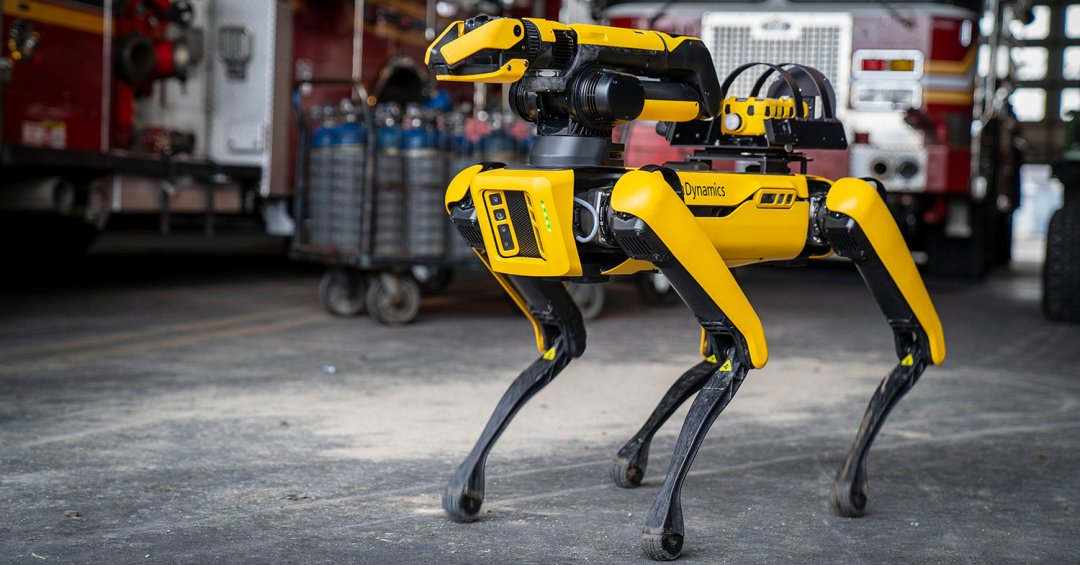
\includegraphics[scale=.5]{boston-dynamics-spot}
    \caption{Spot an agile multipurpose robot from Boston dynamics} 
\end{figure}
However, developing the technologies necessary for autonomous robots is a formidable undertaking with deep interweaved ramifications in automated reasoning, control and perceprion, which raises many important problems, one of them which is \textbf{motion planning}, which is the major theme of this project work. Since we live in a dynamic and unpredictable environment it is not possible to explicitly describe all the possible motions that a robot may have to exeecute in order to accomplish a requested task. Hence the need for algorithms 

This work focus on the topological study of robot motion planning algorithms using results from algebraic topology and some other important areas of mathematics, and we also give pratical computational simulation of robotic manipulator using the C++ and Python programming languages, the robotic operating system (ros) and Gazebo virtual robot simulator running on an Ubuntu Linux machine.

%%%%TODO add the references to each of the mentioned works
\section{Literature Review}
Motion planning is a fundamental problem in robotics. It is the problem of finding a safe and efficient path for a robot to move from one point to another in its environment. The environment may be cluttered with obstacles, and the robot may have limited mobility. Motion planning is a challenging problem, and there is no single algorithm that can solve all cases.

The study of Topological robot motion planning started in 2003-2004 by Michael Farber. His motivation was using tool from algebraic topology, whereby he considered a path connected topological space whose path space is equipped with the compact open topology. Using this the motion planning algorithm of any mechanical robot that moves in a configuration space is represented to be the funcion of input and output with the input being the two points (that is the current location of the robot and its destination) and the output is the path to be taken by the robot.

In the earlier work of Farber he introduces an homotopy invariant called Topological complexity, which measures the minimum number of continuous motions required to move a robot from one configuration to another in a given configuration space. In this founding paper he was only concerned with the departing motion of the robot and not the returning motion, but made up for this in a subsequent work with M. Grant where the concept \textit{symmetric topological complexity} was introduced. This studies when the departing and returning motion of the robot are the same.

Using the motivation of Farber and Grant, Mamouni and Derfourfi considered the case when the robot is allowed to take any arbitrary path to come back to its departure point, as in the case of the motion of drone, or an unmanned air-plane, or a guided TV camera, they studied homotopically and topologically the concept of \textit{loop motion planning algorithm (LMPA)}  and define the \textit{loop topological complexity} which is a generalization of the work of Farber and Grant.

Mamouni and Derfoufi uses the F\'elix-Thomas generaization of the Chas-Sullivan \textit{String topology} into rational homotopy to make generalization of \textit{string topology} into a broad topological robotics settings.

\section{Some Basic definitions}
In this section we introduced the basic definitions to be used the next sections and chapters of this project work.

\begin{defn}[Topological Space]
    Let $X$ be a nonempty set and $\tau$ be the collection of open subsets of $X$ satisfying the following conditions
    \begin{itemize}
        \item[1.] $\emptyset, X \in \tau$
        \item[2.] the union of every class of set in $\tau$ is a set in $\tau$
        \item[3.] the intersection of every finite class of sets in $\tau$ is a set in $\tau$
    \end{itemize}
    $\tau$ is called the topology on $X$ and the ordered pair $(X, \tau)$ is called a topological space. When $\tau$ is out of context we use ordinary $X$.
\end{defn}

\begin{defn}[Subspace]
    Let $(X, \tau)$ be a topological space and\\
     $Y \subset X$ be nonempty.\\
    The relative topology or subspace topology on $Y, \tau_Y$ is defined as the class of all intersections with $Y$ of open sets of $Y$
    \[
        \tau_Y = \{Y \cap U  \mid U \in \tau\}
    \]
    The pair $(Y, \tau_Y)$ is called a topological subspace of $(X, \tau)$.
\end{defn}

\subsubsection*{Some examples of topological spaces}
\begin{enumerate}
    \item Let $X = \{x,y,z\}$ and $\tau = \{X, \emptyset, \{x\}, \{x,y\}, \{x,z\}\}$. Then $(X, \tau)$ is a topological space.
    \item For any nonempty set $X$, let $\tau$ be the class of all  subsets of $X$. Then $(X, \tau)$ is a topological space.
\end{enumerate}

\begin{defn}
    Let $X$ be a topological space and $x \in X$ 
    \begin{enumerate}
        \item An open neighbourhood of $x$ is an open subset of containing $x$.
        \item A neighbourhood of $x, N(x)$ is a subset of $X$ containing an open neighbourhood. i.e. N (x) is a neighbourhood of x if there exists an open set Q such that $x \in Q \subset N (x)$.
        \item The class of all neighbourhoods of $x \in X$ denoted by $N_x$ is called the neighbourhood system of x.
    \end{enumerate}
\end{defn}

\begin{defn}[Continuous functions]
    Let $X,Y$ be topological spaces and \\
    $\disp f: X \lra Y$ is a mapping, $f$ is said to be continuous if $\disp f^{-1}(G)$ is open in $X$ whenever $G$ is open in $Y$.

    That is, for $(X, \tau_1),(Y, \tau_2,), f$ is continuous if $f^{-1} (G) \subset \tau_1$ whenever $G \in \tau_2$ or the inverse image of an open set is open under a continuous function.
\end{defn}

\begin{defn} 
    Let $X$ be a topological space.
    \begin{enumerate}
        \item A class $\{G_i\}$ of open subsets of $X$ is said to be an open cover of $X$ if each point of $X$ belongs to at least one $G_i$. That is, $\{G_i\}$, a collection of open sets is a cover for $X$, if $X = \cup_{i \in I} G_i$.
        \item A subclass of an open cover of $X$ which itself is an open cove is called a \textit{subcover}.
        \item An open cover (or subcover) is \textit{finite} if it contains finitely many elements. 
    \end{enumerate}
\end{defn}

\begin{defn}[Compact space]
    A compact space is a topological space $X$ in which every open cover $\{G_i\}_{i \in I}$ of $X$ has a finite subcover. That is, there exists $G_1, \ldots, G_n \in \{G_i\}_{i \in I}$ so that $X  = G_1 \cup \ldots \cup G_n$ 
\end{defn}

\begin{defn}[Regular space]
    A topological space $X$ is said to be regular if it has the property that if $x \in X$ and $F$ any closed subspace of $X$ such that $x \notin F$, there exists disjoint open sets $U,V$ such that $F \subset U$ and $x \in V$. That is, it is always possible to separate $x$ and $F$ with disjoint open sets, when $x \notin F$.
\end{defn}

\begin{defn}
    Let $X$ be atopological space 
    \begin{enumerate}
        \item A separation of $X$ is a pair $U,V$ of open subsets of $X$ whose union is $X$.
        \item $X$ is said to be connected if it cannot be represented as the union of two disjoints open sets. That is there doesnot exist a separation of $X$.
    \end{enumerate}
\end{defn}

\begin{defn}[Path]
    Given any points $x,y$ in a topological space $X$, a path in $X$ from $x$ to $y$ is a continuous function $\alpha : [0,1] \lra X$ with $\alpha(0) = x$ and $\alpha(1) = y$, since we can rescale it to $\beta(t) = \alpha((b-a)t + a)$ for $t \in [0,1]$
\end{defn}
\begin{defn}[Path-connectedness]
    A path connected space is a topological space $X$ in which for any points $x,y \in X$ there exists a path in $X$ from $x$ to $y$.
\end{defn}

\begin{defn}[Homotopy]
Let $X$ and $Y$ be two topological spaces, let $f,g : X \lra Y$ be maps and $I = [0,1]$. Then the \textit{homotopy} from $f$ to $g$ is the map $F: X \times I \lra Y$ such that $F(x,0) = f(x)$ and $F(x,1) = g(x)$ for all points $x \in X$.
\end{defn}

\begin{notn}
If $F$ is the homotopy from $f$ to $g$ we write $\disp f \htp{F} g.$
\end{notn}

\begin{defn}[Homotopy Type]
Two spaces $X$ and $Y$ have the same homotopy type (or are homotopy equivalent, or homotopic), if there exists maps $f: X \lra Y$ and $g : Y \lra X$ such that $g \circ f \simeq 1_X$ and $f \circ g \simeq 1_X$
\end{defn}

\subsection*{Examples of Homotopic spaces}
\begin{enumerate}
\item All homeomorphic spaces are homotopic.
\item Any convex subset of a Euclidean space is homotopic to a point.
\end{enumerate}

\begin{defn}[Contractible space]
A space $X$ is called contractible if the identity map $1_X$ is homotopic to the constant map at some point of $X$.
\end{defn}